\section{Parsing and syntax trees}
\label{sect:parser_and_syntaxtrees}
The act of parsing is the process of analyzing a series of tokens and construct
a grammatical structure (syntax tree) based on a formally specified grammar. In
figure \ref{figure:parser:overview}, the parser component of a generic
compiler/interpreter is shown. 

\begin{figure}[h]
  \centering
    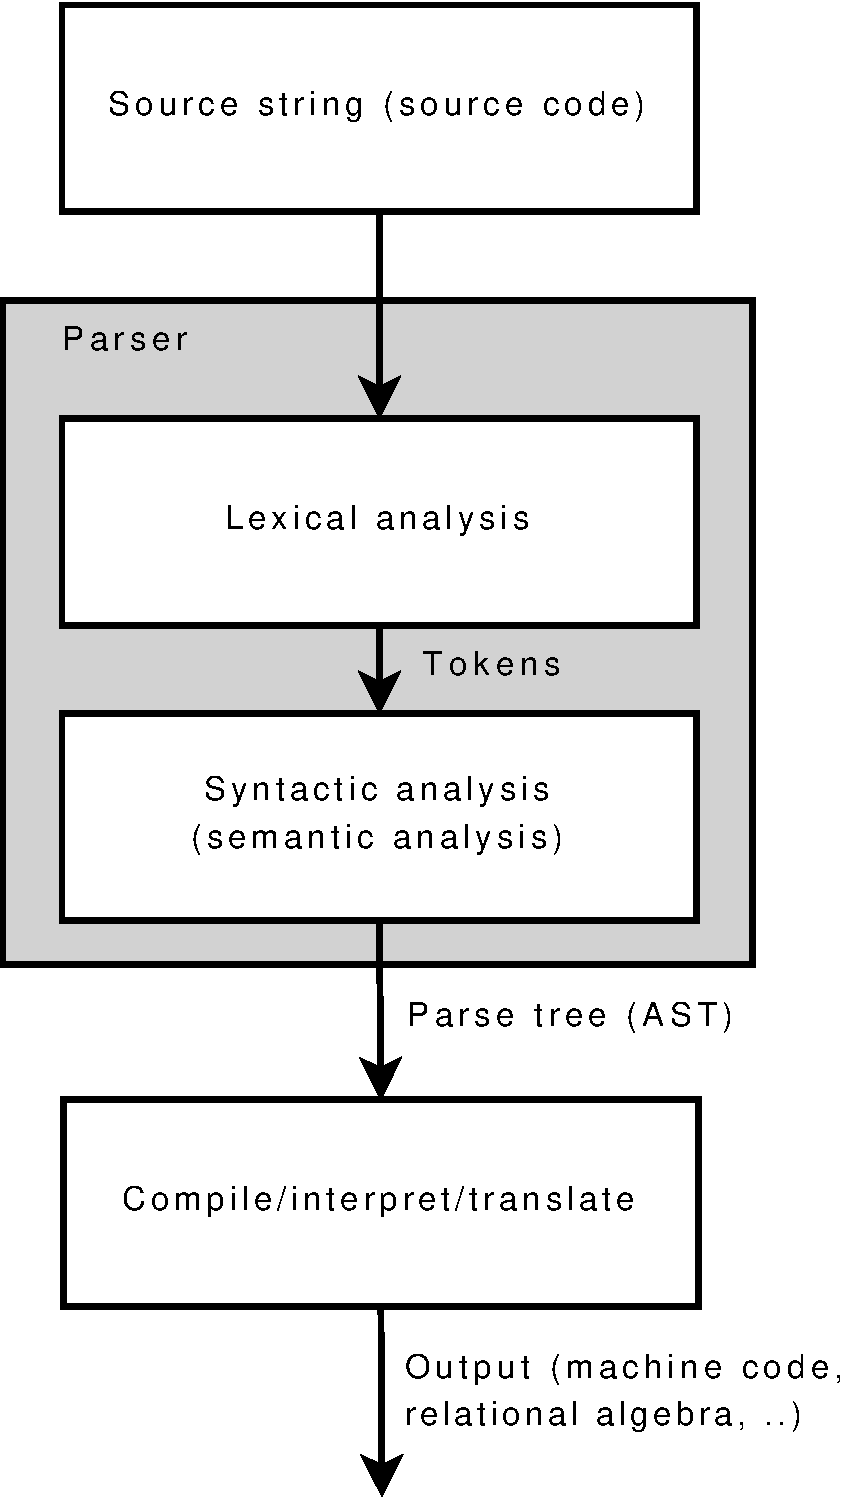
\includegraphics[scale=0.40]{diagrams/parser_overview}
  \caption{Typical compiler/interpreter data flow}
  \label{figure:parser:overview}
\end{figure}

\subsection{Common parser technologies}
There are two common types of parser technologies, \textit{top-down} and
\textit{bottom-up} parsers. As their names imply, these technologies differ in
the sense that top-down parsers will attempt to match production rules with the
input top-down, while bottom-up parsers will start with the terminal symbols and combine them into production
rules. Often this is implemented as a process of shift and reduce operations utilising stacks to hold
production rules and terminal symbols.\marginpar{\textbf{\Large TODO}\scriptsize Holder de production rules eller
noe som er matcha?}

We refer to \cite{compiler_tech} for further in-depth information about parser
technologies. However, it is important to note that typically a top-down parser
based on an LL\footnote{LL is a Left-to-right, Leftmost derivation
parser, using a top-down approach}-grammar with low token lookahead (typically
one token lookahead, aka LL(1)) will perform better and be subject to a high
number of well-defined optimisations, out of which a few are described in
\cite{compiler_tech} and \cite{DBLP:books/cu/Appel1998c}.\marginpar{\textbf{\Large TODO}\scriptsize skjonte ikke
helt, er LL bedre enn LALR? eller LL(1) bedre enn LL(2)?}

\subsection{Parser generators}
For large grammars, writing a parser by hand from the ground up may turn out to
be a substantial amount of work. To eliminate this, a large number of
parser generators exist. Most of these parser generators have a very
similar set of functionality. From a formal grammar, often in a notation
similar to BNF, the parser generator will output the source code for a
complete parser for the given grammar. Ideally, the maintainability of this
generated parser could be reduced to simply changing the grammar specification,
without actually modifying the generated source code.

\begin{figure}[h]
  \centering
    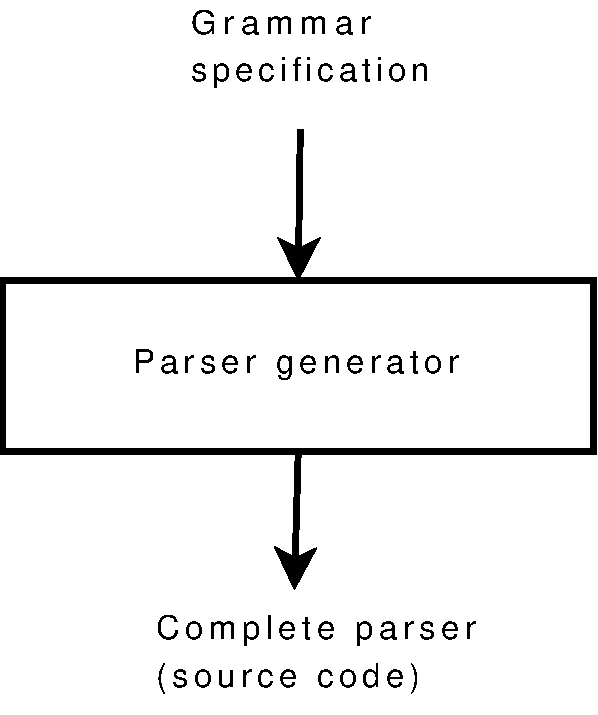
\includegraphics[scale=0.40]{diagrams/parser_generator}
  \caption{Automatic parser generation workflow}
  \label{figure:parser:generator}
\end{figure}

Several parser generators exists, covering several target languages and
overlapping in terms of functionality and features. As expected, the most
common parser generators will generate either top-down or bottom-up parsers. Typical examples of bottom-up parser
generators are yacc (and derivatives), CUP, GOLD, and SableCC. Some popular
top-down parser generators include JavaCC, ANTLR, Spirit, and Coco/R.

A comparison of some of the most popular parser generators were made in
\cite{ourselves} for the development of the XQFT Parser (see section \ref{sect:theory:xqftparser}), and out of
these the ANTLR parser generator was chosen. We will not reiterate the features of ANTLR in this document, however
it is important to note that ANTLR can generate predicated LL(*)-parsers\cite{definitiveAntlr} based on
LL-compliant grammars. This choice was made due to the XQuery BNF specification
which is claimed to be LL(1) (one token lookahead) -- however, as discussed in
\cite{ourselves}, it may not be suitable to define the required lookahead for this grammar, as it contains
ambiguities.

\subsection{The XQFT Parser project}
\label{sect:theory:xqftparser}
The XQFT Parser\cite{ourselves} was developed as a part of an academic project
at the Department of Computer and Information Science (IDI) at the Norwegian
University of Science and Technology (NTNU) throughout the autumn of 2007.

In this project the ANTLR parser generator was utilised to generate a
predicated LL-parser based on the W3C specification\cite{w3c01} for XQuery with
full-text extensions.

The output from this parser are carefully crafted abstract syntax trees which
are well suited for translation into other representations.

% The data flow for the generation of the XQFT Parser is shown in figure
% \ref{fig:parser:xqft_antlr_gen} where the grammar is input, and the ANTLR
% parser generator produces the XQFT Parser.
% 
% \begin{figure}[!htp]
% \begin{center}
%   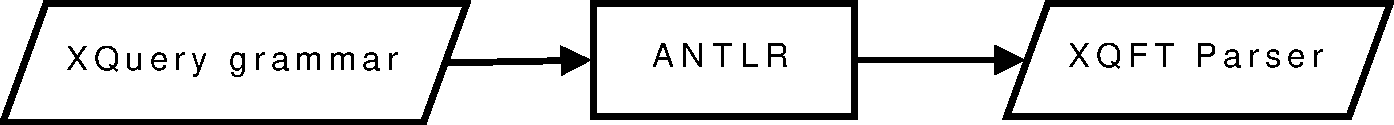
\includegraphics[scale=0.5]{diagrams/xqft_antlr_dataflow}
%   \caption{Data flow for generation of the XQFT Parser}
%   \label{fig:parser:xqft_antlr_gen}
% \end{center}
% \end{figure}

The dataflow for actual use of the XQFT parser is shown in figure
\ref{fig:impl:sys:mql_dataflow} on page \pageref{fig:impl:sys:mql_dataflow}.

\subsubsection{AST construction}
\label{sect:theory:xqftparser:ast_construction}
The abstract syntax tree is constructed by specifying tree rewrite rules in the
grammar file (the tree rewrite rules is extensively covered in \cite{ourselves}, section
4.5). The tree consists of nodes instantiated from the
\verb!no.ntnu.xqft.parse.XQFTTree! class. To compensate for missing tokens to
determine tree context, the XQFT Parser employs the use of imaginary tokens.
These are simply tokens that do not exist in the input stream, they only have
an associated name and no specific token. These imaginary tokens are typically
used where there are no ``real'' tokens available to represent the proper
semantic or contextual meaning.

One example can be seen in figure \ref{figure:parser:imaginary_tokens_path},
where imaginary tokens, identified by a AST\_-prefix, have been injected into the tree.

\begin{figure}[h]
  \centering
    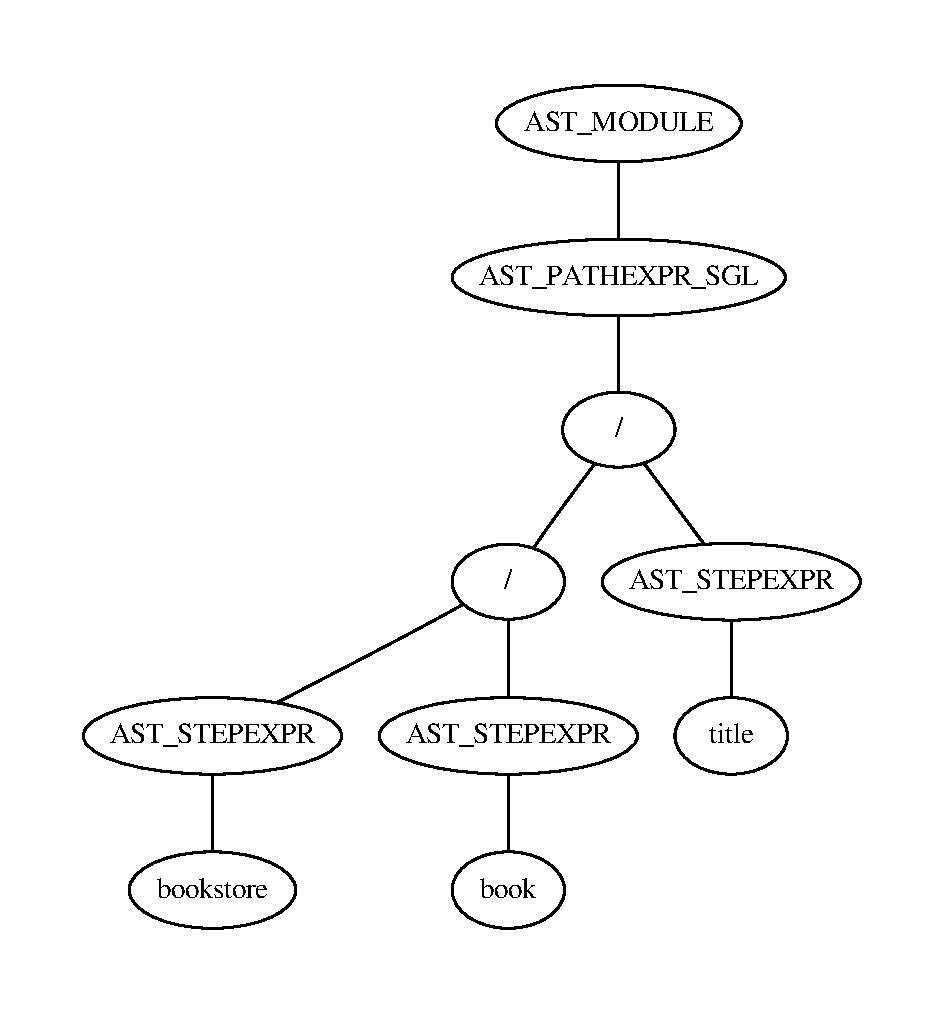
\includegraphics[scale=0.50]{img/graphs/path1} 
  \caption{Example of injected imaginary tokens}
  \label{figure:parser:imaginary_tokens_path}
\end{figure}

\subsection{Tree parsing}
\label{sect:theory:parser:tree_parsing}
Tree parsing (or tree walking) is an integral part of translation from AST to
new structures and representations. Several methods exist to accomplish this in
various manners. Some are restricted by language limitations, while others are
mostly transparent to programming paradigms and syntax. In this section we will
present a small selection of common patterns, and describe their various traits.

\subsubsection{Manual tree walker (non-visitor)}
\label{sect:theory:manual_walker}
One of the simplest forms of tree parsing is the ``manual non-visitor''
methodology. This way of parsing a tree structure is particularly suited for
trivial trees where context is not important. However, for operations that are
contextually sensitive -- such as context-sensitive code generation, as is the
case for this project -- this methodology can be difficult to maintain as the
problem domain expands. This particular problem is rooted in that any
contextual information must be extracted from parent nodes, and is thus not
available implicitly.

Another problem with this technique is that the data structure (the tree) and
the logic to parse it will often be tied together quite closely, creating
another maintanence problem when/if the tree structure changes to
accommodate new specifications.

\subsubsection{Visitor pattern}
\label{sect:theory:visitorPattern}

\begin{figure}[h]
  \centering
    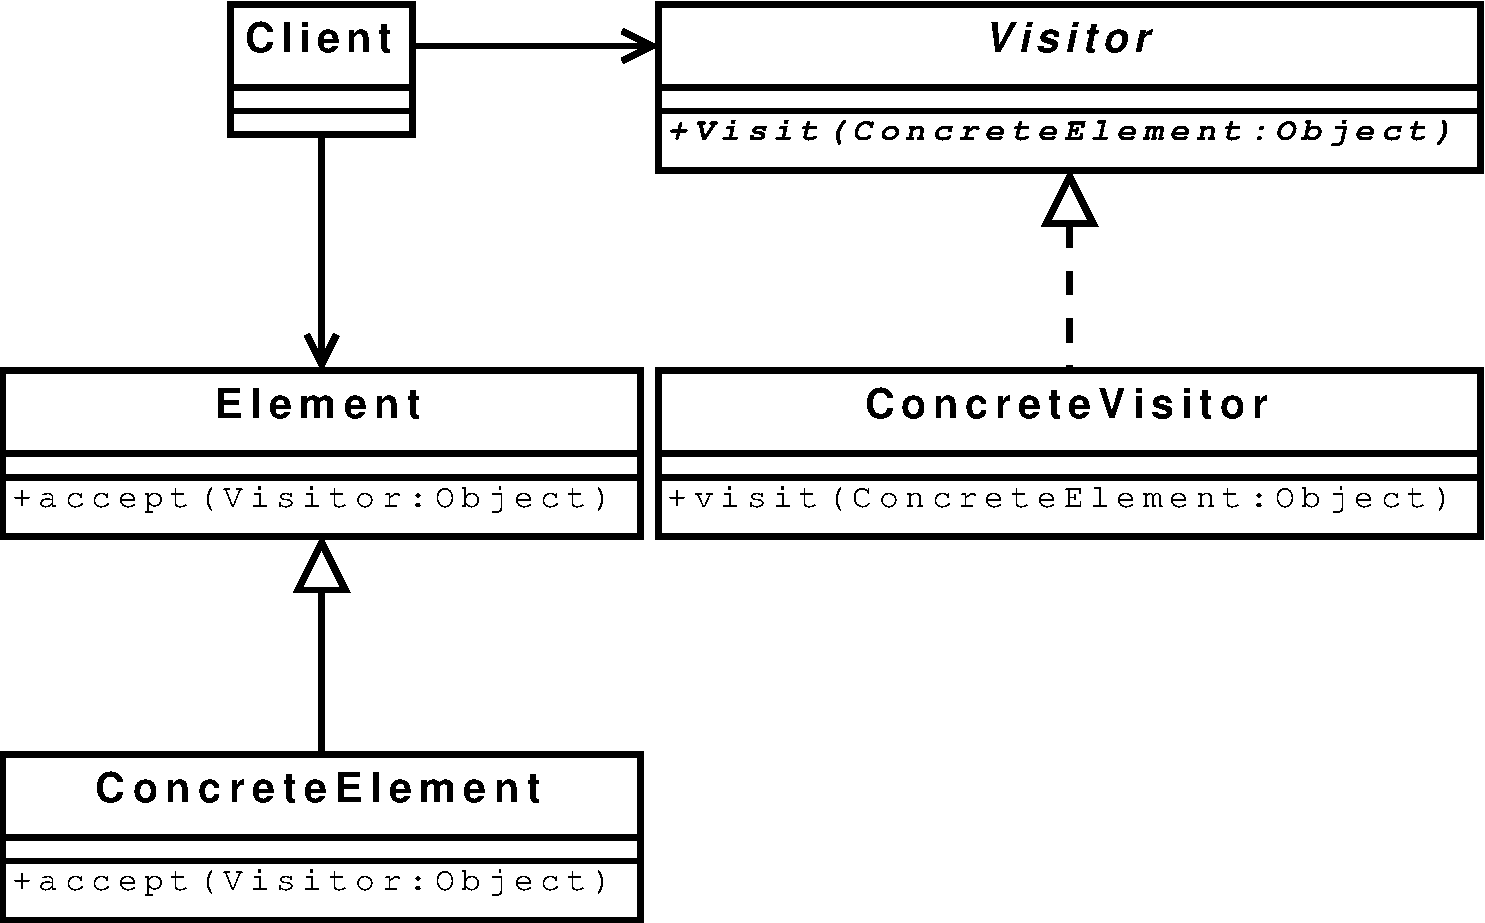
\includegraphics[scale=0.40]{diagrams/visitor_pattern} 
  \caption{Visitor pattern UML schema}
  \label{figure:parser:visitor_pattern}
\end{figure}

The visitor pattern\cite{agile_software} is a common design pattern for parsing
tree structures. The visitor pattern gives a number of ways to modify the
behaviour of a hierarchy of classes without having to change those classes.
Additionally, this allows the benefit of a clean separation of logic/algorithms
and data structures.

However, the visitor pattern does not scale well with complexity of the problem
domain. In particular, for context-sensitive parsing of tree structures, the
visitor pattern will quickly lead to complex visitors, cluttered with
additional logic for state preservation and determining types.  

\subsubsection{Context-sensitive visitor pattern}
\label{sect:theory:contextVisitorPattern}
Here we present a novel pattern based on the visitor pattern which seeks to
avoid complex state preservation mechanisms and logic for type switching. This idea
is loosely based on the ``island grammar'' concept\cite{islandGrammar}\footnote{See
http://www.program-transformation.org/Transform/IslandGrammars for a brief
introduction}.

The semantics of the context-sensitive visitor pattern can be captured in the
following two rules:
\begin{itemize}
  \item For a change of state which affects how a visitor should behave when
  encountering some node in the subject tree, switch to another visitor which
  incorporates this logic (use inheritance as necessary), and execute this
  visitor on the subject tree
  \item For type switching logic which depends on context in the subject tree,
  switch to another visitor which incorporates this logic (use inheritance as
  necessary), and execute this visitor on the subject tree
\end{itemize}

Simplifying this idea, it means that visitors are specialized and used
interchangeably on the subject tree as needed. This leads to the benefit of
encapsulating state mechanisms and type switching logic in specialized
visitors, thus avoiding a single large and complex visitor.

\begin{figure}[h]
  \centering
    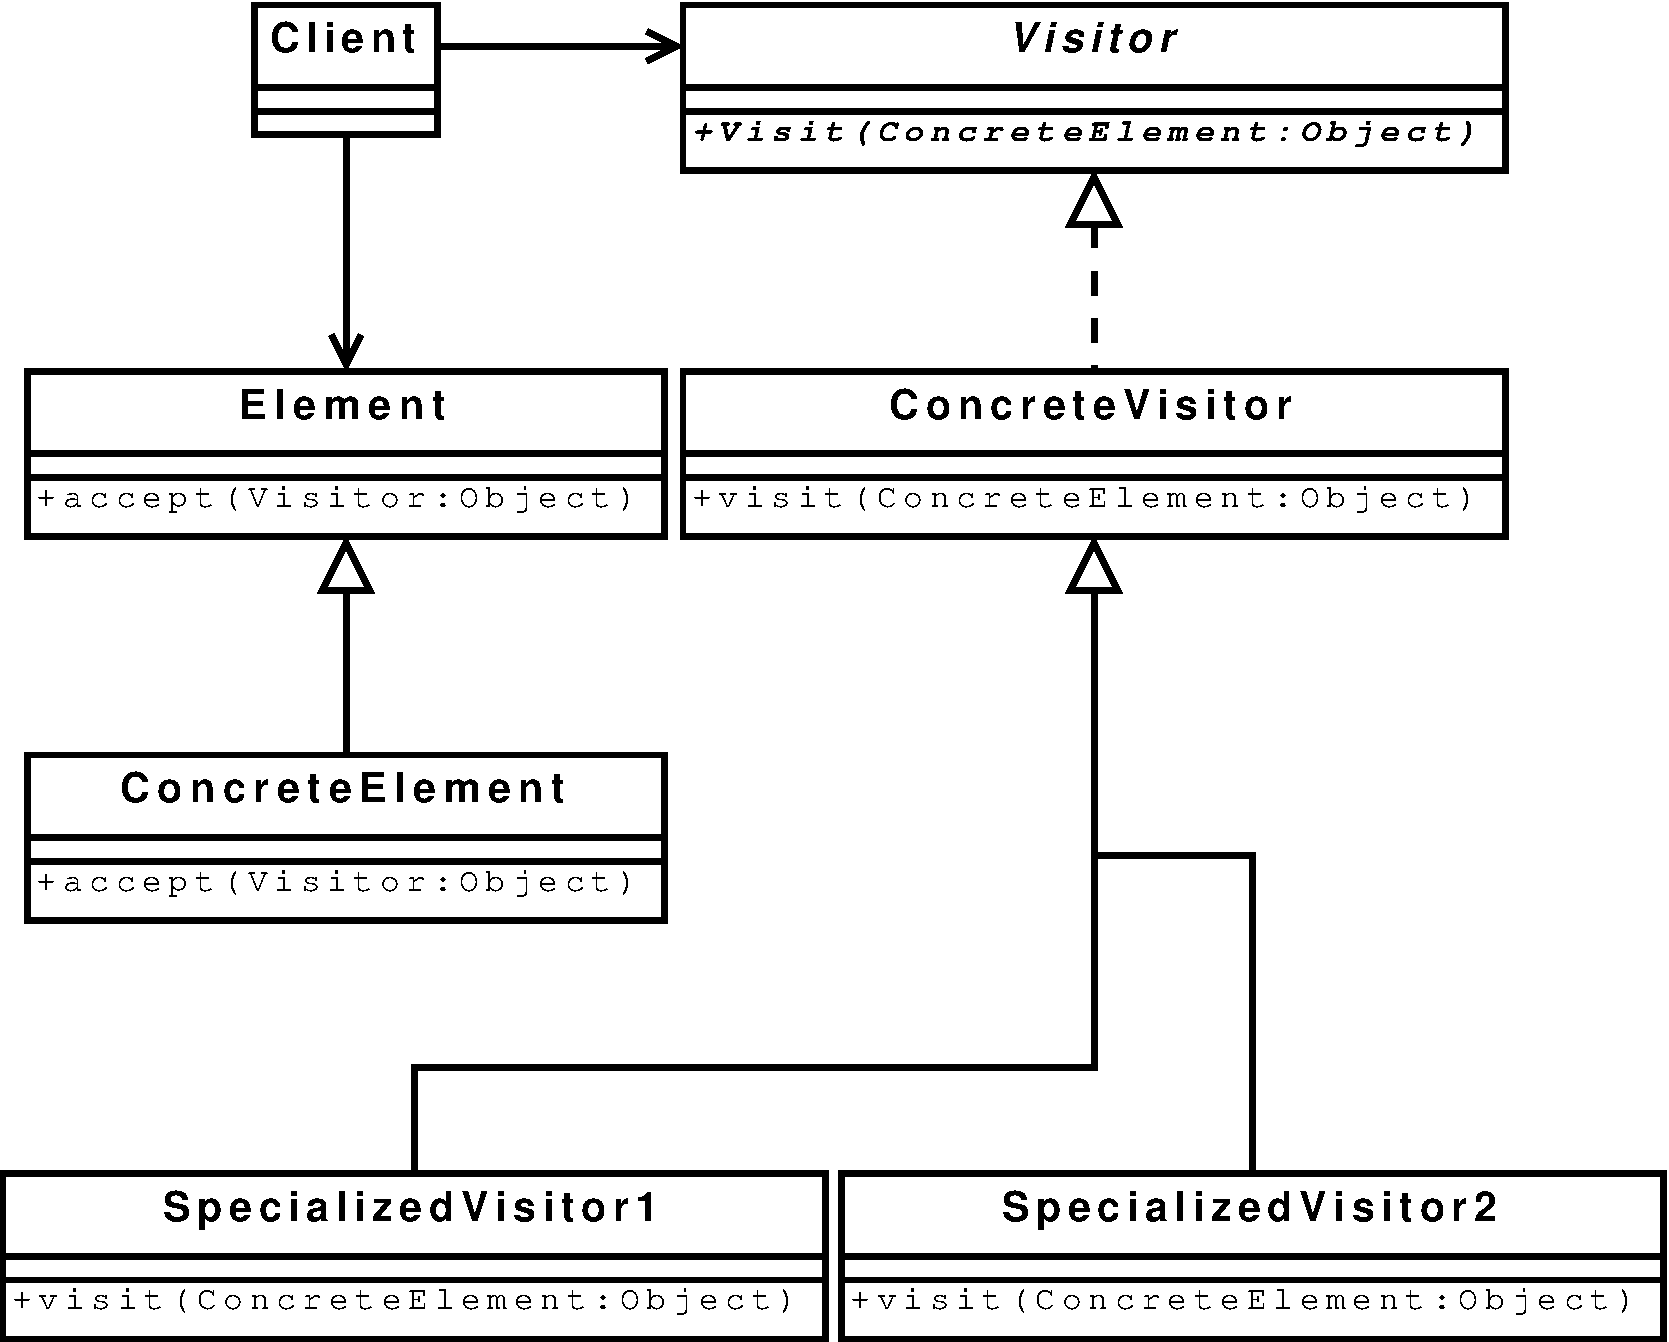
\includegraphics[scale=0.40]{diagrams/context_visitor_pattern} 
  \caption{Context-sensititive visitor pattern UML schema}
  \label{figure:parser:context_visitor_pattern}
\end{figure}

As can be seen in figure \ref{figure:parser:context_visitor_pattern}, the
class structure is similar to a common visitor pattern (figure
\ref{figure:parser:visitor_pattern}). The important distinction thus lies in
the logic and how the visitors are executed and how they interact. The two
classes \verb!SpecializedVisitor1! and \verb!SpecializedVisitor2! are
special-purpose visitors that can be executed from any of the others.
Inheritance is implemented in this example, but is purely optional, as
previously mentioned.